The dipole polarizability of an atom corresponds to the zero-frequency limit of a two-photon process.\(AE\) describes the energy shift of an atom in a static electric field according to
\begin{equation}
    AE = \frac{1}{2}\alpha_\alpha F^2
\end{equation}
Where \(F\) is the field strength. In this chapter we develop computational methods that will be applied later to two photon processes. The dipole polarizability is defined by the second-order perturbation expression\cite{variational}.
\begin{equation}
    \alpha_{d}\equiv- E^{(2)}=-\sum_{n=1}^{N}\frac{\abs{\bra{np}eFr\cos{\theta}\ket{1s}}^{2}}{E_{1s}-E_{n}}
\end{equation}

The hyperfine transition that is being studied is a two photon process where the jump from the ground state to the excited state is mediated by a transition to an intermediate virtual state. This is represented as a summation over all possible states and an integration over the continuum. These two photons can be any frequency so long as the sum of their energies is equal to the total transition energy\cite{loudon}. There is no conservation of energy needed with regards to the intermediate states as no real transitions are occurring\cite{loudon}

\begin{center}

        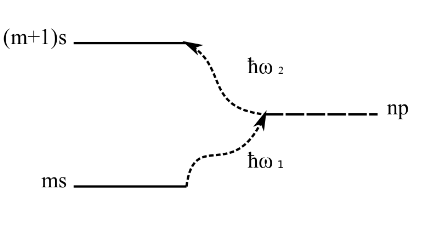
\includegraphics[width=0.4\textwidth]{images/transitioncrop.PNG}

\end{center}
        
In this particular example as our ground state is the \(1s\) state our intermediate virtual states are represented by the p states, as they are the only transitions allowed by parity. The classic method of solving this involves a summation over the entire spectrum of p states and then an integration of the positive continuum. This however is time consuming to do in practice. We instead will be using the pseudo-state method along with the variational method to deal with this.
	The main bulk of using this method is generating the pseudo states, to do this we first define what sort of function we wish to use. For our purposes we found that it is best to work in spherical coordinates as this makes the resulting integrals rather elegant to solve analytically. Every state is expanded in the basis set of functions \(r^n e^{-\alpha r}Y_l^m(\theta,\phi)\)\cite{shark}
	\begin{equation}
    \Psi(r)=\sum_{n=1}^{m}c_{n}r^{n}e^{-\alpha r}Y_{l}^{m}(\theta,\phi)
    =\sum_n c_n \chi_n
    \end{equation}
    \begin{equation}
        \chi_n=r^n e^{-\alpha r}Y_l^m(\theta,\phi)
    \end{equation}
    Where \(c_{n}\) is a linear variational parameter and \(\alpha\) is our nonlinear variational parameter. We use this particular form for our wave equations because the integrals can be solved analytically and rather simply.
    \begin{equation}
        \int_{0}^{\infty}r^{n}e^{-\alpha r}dr=\frac{n!}{\alpha^{n+1}}
    \end{equation}
 Firstly we must create out basis set by forming linear combinations. We do this by generating an overlap matrix whose elements are\cite{shark}.
 \begin{equation}
     \chi_{n}(r)=r^{n}e^{-\alpha r}Y_{l}^{m}(\theta,\phi)
 \end{equation}
 \begin{equation}
     O_{mn}=\bra{\chi_{m}}\ket{\chi_{n}}
 \end{equation}
  The way this matrix is orthogonalized is by the Jacobi method, which works in this case because our matrix is symmetric. For our matrix \(O\) we find the largest off diagonal element \(O_{nm}\). We then transform our matrix using a rotational matrix \(Q\) where\cite{jacobi}.
   \begin{equation}
     Q=\begin{bmatrix}
     1  &       &          &          &          &          &  \\
        &\hdots &          &          &          &          &  \\
        &       & \cos{(\theta)}  &\hdots   &-\sin{(\theta)}     & & \\  
        &       &\vdots &1      &\vdots & & \\  
                &       &\sin{(\theta)}   &\hdots   & \cos{(\theta)} & &\\
          &&&&&\hdots  \\    
            & & & & & &1
    \end{bmatrix}
 \end{equation}
  \begin{equation}
      \tan(2\theta)=\frac{O_{nm}}{O_{nn}-O_{mm}}
  \end{equation}
  This transformation is performed iteratively until all of the off diagonal elements are sufficiently small. We then set the total transformation matrix to \(T\) such that.
  \begin{equation}
      T=\prod_{i} Q_{i}
  \end{equation}

and
\begin{equation}
     T^{T}OT=\begin{bmatrix}
     I_{1}       & 0      & 0      &\hdots   & 0     \\
     0           & I_{2}  & 0      &\hdots   & 0     \\
     0           & 0      & I_{3}  &\hdots   & 0     \\  
    \vdots       & \vdots &\vdots  &\ddots   &\vdots \\  
     0           & 0      & 0      &\hdots   & I_{n} 
    \end{bmatrix}
 \end{equation}
Once the matrix is diagonalized we then apply a scalar change matrix to transform it to the identity matrix as follows
\begin{equation}
    S=\begin{bmatrix}
     \frac{1}{I_{1}^{\frac{1}{2}}}       & 0      & 0      &\hdots   & 0     \\
     0            &  \frac{1}{I_{2}^{\frac{1}{2}}}  & 0      &\hdots   & 0     \\
     0            & 0      &  \frac{1}{I_{3}^{\frac{1}{2}}}  &\hdots   & 0     \\  
     \vdots       & \vdots & \vdots  & \ddots  & \vdots \\  
     0            & 0      & 0       &\hdots   & \frac{1}{I_{n}^{\frac{1}{2}}} 
    
    
    \end{bmatrix}
\end{equation}
Where
\begin{equation}
    S^{t}T^{T}OTS=1
\end{equation}
We combine the two transformations as \(R=TS\) so that.
\begin{equation}
    R^{T}OR=1
\end{equation}
Once total transformation matrix is generated we then generate the Hamiltonian matrix of the form \(H_{nm}=\bra{\psi_{m}}H\ket{\psi_{n}}\) which we then express in our new basis set using our transformation matrix as follows
\begin{equation}
    H^{\prime}=R^{T}HR
\end{equation}
We then diagonalize our resulting matrix to give us our eigenvalues and eigenvectors for our basis set by applying an orthogonal transformation W.
\begin{equation}
    W^{T}H^{\prime}W=\begin{bmatrix}
    \lambda_{1} &0             &\hdots    &0 \\
    0           &\lambda_{2}   &\hdots    &0 \\
    \vdots      &\vdots        &\ddots    &\vdots \\
    0           &0             &0         &\lambda_{n}
    
    
                     \end{bmatrix}
\end{equation}
Our eigenvectors are given by applying our transformation matrices to the original wave equations, with the combination of R and W giving rise to the overall scale factor.
\begin{equation}
    \Psi^{q}(r)=
    \sum_{n,n^{\prime}}r^{n}e^{-\alpha r}Y_{l}^{m}(\theta,\phi)R_{n^{\prime},n}W_{n,q}
\end{equation}

Now that we have our new basis set we will be applying it to the calculation of the polarizability of hydrogen. We use the scenario of a hydrogen atom in the ground state within a static electric field of strength \textit{F} pointing in the \textit{z} direction. This gives rise to the perturbation of \(V=eFr\cos{\theta}\). Since we are working with hydrogen, the first order perturbation to the wave equations can be solved analytically. However this is a test of our pseudo-state method so we will be using that instead to calculate our second order correction to the energy. This is useful because we can use this very simple example to prove that our method works and can be applied to much more complex examples. Our pseudo-states \textit{n} will be applied in the following way to calculate the second order correction to the energy.
\begin{equation}
    E^{(2)}=\sum_{n=1}^{N}\frac{\abs{\bra{n_{p}}eFr\cos{\theta}\ket{1_{s}}}^{2}}{E_{1{s}}-E_{n}}
\end{equation}
Taking this with the definition of the dipole polarizability
\begin{equation}
    \alpha_{d}\equiv- E^{(2)}=\frac{9}{2}a_{0}^{3}
\end{equation}
We arrive at the correct answer of \(4.5a_{0}^{3}\).

There are several things worth mentioning about this technique. Firstly our variational parameter \(\alpha\). If we were to take our function for the dipole polarizability with a small basis set and plot is as a function of \(\alpha\) we can see that there is a rather significant variance. However we can very plainly see an absolute maximum located at \(\alpha=1\)\cite{variational}.  We can also see that there is an upper bound to our function and no matter how large we expand our basis set that ceiling of the true value of \(4.5a_{0}^{3}\) remains.

The one important thing that does change is our range of \(\alpha\) that will give us that result, as the functions ceiling tends to smooth out for larger basis sets as it is pressed against the true value. What this means is that, the larger our basis set, the more inaccurate our value for \(\alpha\) can be. When this method is applied to more complicated systems such as helium we can simply expand our basis set to larger and larger values to accommodate for our \(\alpha\). The main drawback is that the larger basis set used, the longer the computation time. Instead a much more economical technique is looking at the fact that our correct answer is located at the absolute maximum for our function. We can vary our \(\alpha\) to find this maximum to arrive at our ideal result. When working with more complicated systems it is far more economical to use these variational parameters find a maximum then it is to create a larger basis set.

For our purposes however we can arrive at our result of \(4.5a_{0}^{3}\) using only a two dimensional basis set\cite{variational}. This is extremely powerful as we are representing the entire spectrum of hydrogen with only two wave equations, greatly reducing our computing time.



